
\begin{itemize}
	\item The creatioon of Lender-Criteria bipartite graphs
	\item Explain why we could not project Lender-Criteria graphs onto Lender to create Lender-Lender graph
	\item That's why we find communify directly in bipartite graphs
	\item Methodology: better-than-random testing
\end{itemize}

\section{Hypothesis testing on syntehsis data}

\begin{itemize}
	\item How to build a random graph, with community pre-defined
	\item Detecting community in random graph
	\item Quality assessment of the detected community, presented by a numer $Q_{synthesis}$
	\item $Q_{synthesis}$ gives an idea about the best we could get from a data, but depends on the laten parameters when building datasets $p_{in}$, $p_{out}$, $p_{change}$ - the change from community to another
\end{itemize}

\section{Hypothesis testing on real data}

\begin{itemize}
	\item Filter data to keep Lenderes who is active invest from 2019-2023
	\item Repeat the works on random graph for each year data
	\item Then find quality assessment $Q_{real}$ again and compare with $Q_{synthesis}$.
	      Decide if there is a clear community for different criteria (Tags, Sectors, Country)
\end{itemize}

As the begin of this chapter, we are revisiting our hypothesis and testing them out.
Recall that we would like to find community of Lenders, based on their interests in different criteria.
Through the data explornation, we will use 3 different criteria to find if the community exists.
The criteria are: Tags, Sectors and Country.

The first steps is to associate each Lender with Criteria.
In the Kiva data, Lender and Criteria are connected through the Project.
A Lender is considered to be interested in a Criteria if he/she has invested in a Project that has that Criteria.
Note that the relationship between Lender and Project is many-to-many.
The relationship between Project and Criteria could be many-to-many in the case of Tags,
or can be one-to-many in the case of Sectors and Country.
Because of the many-to-many relationship, we will model the data in Graph data type.
This decision is also supported by the fact that the "community finding" is a graph problem.
And by modeling the data in Graph, we can apply the work to other crowdfunding platforms.

\section{Lender-Criteria bipartite graph}

\note{describe about Lender Tags graph, and told that the same apply for Lender sector and lender country}

Like mention above we will use three Criteria features: Tags, Sectors and Country.
But in fact, Lenders do not have any direct relationships with Tags, Sectors or Country.
The relationship between Lender and Criteria is through the Project.
We consider that a Lender choose to invest in a Project because he/she is interested in the Criteria of that Project.
The interests could be explicitly, when a Lender actively find a project with sepecifics crietria.
For example, a Lender who intend to give money to Vietnamese people can search for
all the Projects that have the the Country criteria set to Vietnam.
That feature is available on Kiva website like described in previous chapter.
The interests could also be implicitly, which means that the Lender does not actively search for a Project with specific criteria.
For example, a Lender can contribute to a Project that he or she found on the homepage of Kiva,
and that Project has the Tag "Schooling".
He/she does not actively search for Projects with Tag "Schooling",
yet he/she contributes money to the projects.
We consider that the Lender is interested in the Tag "Schooling".


\begin{figure}[H]
	\centering
	\begin{subfigure}[b]{0.4\textwidth}
		\centering
		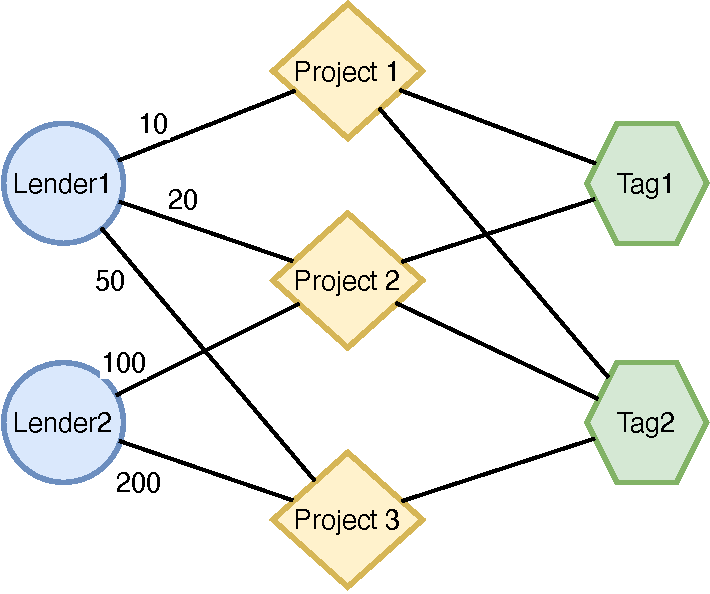
\includegraphics[width=0.8\textwidth]{images/schema_lender_tag.pdf}
		\caption{The relationship between Lender and Tag}
		\label{fig:schema_lender_tag}
	\end{subfigure}
	% \hfill
	\hspace{5mm}
	\begin{subfigure}[b]{0.4\textwidth}
		\centering
		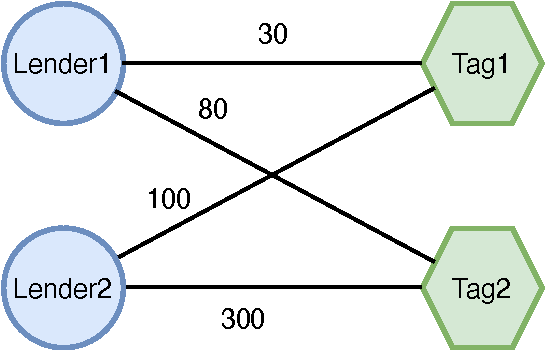
\includegraphics[width=0.6\textwidth]{images/create_lender_tag.pdf}
		\caption{The created Lender-Tag bipartite graph}
		\label{fig:create_lender_tag2}
	\end{subfigure}
	\caption{Process of creating the relationship between Lenders and Tags}
	\label{fig:create_lender_tag}
\end{figure}


Figure \ref{fig:create_lender_tag} illustrate the process of creating the relationship between Lenders and Tags.
For example, Lender1 has invested \$10 to Project1, \$20 to Project2 and \$50 to Project3.
Lender2 contributed \$100 to Project2 and \$200 to Project3.
Project1 was tagged with Tag1 and Tag2, the same for Project2, while Tag3 is the soly Tag of Project3.
We could see that Lender1 express his/her interest in Tag1 through two projects: Project1 and Project2.
We could further "weight" this interest by the amount of money that Lender1 contributed to Projects.
Lender1 contributed \$10 to Project1 and \$20 to Project2,
so we could say that Lender1 interest \$30 in Tag1.
By this way, we could construct a bipartite graph between Lenders and Tags like in Figure \ref{fig:create_lender_tag2}.

We also take this apportunity to mathematically define the notation that we will use in this chapter.
To list all the partites appear in our work, it would be Lender, Project, Tag, Sector and Country.
We will use the full name of the partite to denote the set of nodes in that partite.
For example, $Lender$ is the set of all Lenders.
For each member of each partite, we will use the first letter of the partite to denote the node.
For example, $L_1$ is a node in the set $Lender$.

Denote the graph in figure \ref{fig:schema_lender_tag}
\begin{equation}
	LPT(Lender, Project, Tag, LEND, TAGW)
\end{equation}

Where

\begin{itemize}
	\item $Lender \triangleq \{L_1, L_2, \ldots, L_i,\ldots \}$ is the set of Lenders. $0 \le i \le |Lender|$
	\item $Project \triangleq \{P_1, P_2, \ldots, P_j,\ldots \}$ is the set of Projects. $0 \le j \le |Project|$
	\item $Tag \triangleq \{T_1, T_2, \ldots, T_k,\ldots \}$ is the set of Tags. $0\le k \le |Tag|$
	\item $TAGW_{j,k}$ is the edges between Project $P_j$ and Tag $T_k$. $TAGW_{j,k} \in \{0, 1\}$
	\item $LEND_{i,j}$ is the edges between Lender $L_i$ and Project $P_j$,
	      It also is the amount of money in US dollar that $L_i$ contributed to $P_j$.
\end{itemize}

Note that the above is a 3-partite graph, which can be view as 2 bipartite graphs.
The first one is between Lenders and Projects

\begin{equation}
	LP(Lender, Project, LEND)
\end{equation}

The second one is between Projects and Tags

\begin{equation}
	PT(Project, Tag, TAGW)
\end{equation}

Denote the graph between Lenders and Tags as

\begin{equation}
	LT(Lender, Tag, INTEREST)
\end{equation}

Where the edge $INTEREST$ between Lender $L_i$ and Tag $T_k$ is the sum of amount of money that $L_i$ contributed to all Projects that have Tag $T_k$.

\begin{equation}
	INTEREST_{i,k}= \sum_{0\le j \le |Project|} LEND_{ij}\times TAGW_{jk}
\end{equation}

Follow the same logic, we could cosntruct the relationship between Lenders and Sectors, and between Lenders and Country.


\todo{create the graph LT, LS, LC and present basic statistics here}

\begin{table}[H]
	\centering
	\resizebox{\textwidth}{!}{%
		\begin{tabular}{|l|r|r|r|r|r|r|r|}
			\hline
			               & $n_1$     & $n_2$     & $m$        & $k_1$            & $k_2$ & $k$  & $\delta$ \\
			\hline
			actor-movies   & 127,823   & 383,640   & 1,470,418  & 11.5             & 3.8   & 5.7  &
			0.000030                                                                                         \\
			authoring      & 19,885    & 16,400    & 45,904     & 2.3              & 2.8   & 2.5  & 0.00014  \\
			occurrences    & 13,587    & 9,264     & 183,363    & 13.5             & 19.8  & 16.0 & 0.0015   \\
			peer-to-peer   & 1,986,588 & 5,380,546 & 55,829,392 & 28.1             & 10.4  & 15.2 &
			0.0000052                                                                                        \\
			kiva LT        & 25        & 63,935    & 282,870    & \textbf{11314.8} & 4.4   &      &
			\textbf{0.177}                                                                                   \\
			kiva LS        &           &           &            &                  &       &      &          \\
			kiva LC        &           &           &            &                  &       &      &          \\
			kiva active LT &           &           &            &                  &       &      &          \\
			kiva active LS &           &           &            &                  &       &      &          \\
			kiva active LC &           &           &            &                  &       &      &          \\                                                                                                  \\
			\hline
		\end{tabular}%
	}
	\caption{\todo{rename graph}}
	\label{tab:bipartites-statistics}
\end{table}

\todo{why it is impossible to project onto Lenders?}

\todo{degree distribution \cite{latapy2006}}


\todo{Transaction to next chapter}

\section{Hypothesis testing on synthesis data}
\section{Hypothesis testing on real data}